%% %%%%%%%%%%%%%%%%%%%%%%%%%%%%%%%%%%% %%
%% Elementos Textuais (Capítulos)      %%
%% %%%%%%%%%%%%%%%%%%%%%%%%%%%%%%%%%%% %%

% Configuração para limpar cabeçalhos e manter apenas número da página
\pagestyle{fancy}
\fancyhf{} % Limpa cabeçalho e rodapé
\fancyhead[R]{\small\thepage} % Número da página no canto superior direito
\renewcommand{\headrulewidth}{0pt} % Remove linha do cabeçalho

% Força o mesmo estilo para todas as páginas (incluindo seções e capítulos)
\fancypagestyle{plain}{\fancyhf{}\fancyhead[R]{\small\thepage}\renewcommand{\headrulewidth}{0pt}}

% Força o mesmo estilo para páginas de capítulos
\fancypagestyle{chapter}{\fancyhf{}\fancyhead[R]{\small\thepage}\renewcommand{\headrulewidth}{0pt}}

% Força o mesmo estilo para páginas de seções
\fancypagestyle{section}{\fancyhf{}\fancyhead[R]{\small\thepage}\renewcommand{\headrulewidth}{0pt}}

%% Inclua aqui os capítulos que farão parte do TCC
% ----------------------------------------------------------
% Introdução
% ----------------------------------------------------------
\chapter{Introdução}

% Contextualização 

Em um país de dimensões continentais como o Brasil, o transporte rodoviário de passageiros desempenha um papel estratégico na promoção da mobilidade interurbana, conectando municípios e regiões e garantindo o acesso a serviços, trabalho e lazer para milhões de pessoas. Esse serviço, regulamentado pela Agência Nacional de Transportes Terrestres (ANTT), é operado por empresas privadas e possui alta capilaridade, conectando centros urbanos de diferentes portes e promovendo interações espaciais ao longo do território nacional \cite{santos2024}.

A relevância desse modal de transporte fica evidente nos números: em 2019, o sistema interestadual atendeu mais de 2.000 municípios em 25 estados e no Distrito Federal, transportando cerca de 80 milhões de passageiros \cite{santos2024}. Esse volume expressivo de deslocamentos ressalta a necessidade de soluções tecnológicas para modernizar a gestão desse sistema, otimizando a venda de passagens e a administração operacional das empresas de transporte.

% Delimitação do tema

Diante desse cenário, este trabalho propõe o desenvolvimento de uma plataforma baseada no modelo Software como Serviço (\textit{SaaS, Software as a Service}) para a gestão integrada de empresas de transporte rodoviário alternativo, abordando seus impactos na eficiência operacional e na digitalização do setor. Segundo Chong e Carraro (2006, apud Melo et al., 2007), o \textit{SaaS} pode ser definido como "Software implementado como um serviço hospedado e acessado pela Internet" \cite{melo2007software}. Esse modelo permite que empresas utilizem soluções baseadas em nuvem, reduzindo custos operacionais e facilitando a escalabilidade dos serviços, o que pode ser especialmente vantajoso no setor de transporte rodoviário alternativo.

% % Problema

O transporte rodoviário intermunicipal de passageiros no Brasil enfrenta desafios significativos relacionados à adoção e integração de tecnologias avançadas. A ausência de sistemas integrados de gestão e a resistência à inovação tecnológica comprometem a eficiência operacional e a qualidade dos serviços prestados. De acordo com o Relatório de Análise de Impacto Regulatório da Agência Nacional de Transportes Terrestres (ANTT), a incerteza regulatória e a falta de experimentação com novas tecnologias dificultam a modernização do setor \cite{antt2022}.

% % Relevância do tema {Justificativa}
\section{Justificativa}

A modernização do transporte rodoviário alternativo de passageiros no Brasil é essencial para aumentar a eficiência operacional das empresas do setor, garantindo maior acessibilidade e conectividade. A falta de soluções tecnológicas integradas tem limitado o crescimento desse segmento, que opera de forma fragmentada e sem padronização na gestão de frotas e vendas de passagens. A adoção de plataformas \textit{SaaS} pode transformar esse cenário ao digitalizar processos administrativos e operacionais, reduzindo custos e otimizando recursos. Estudos indicam que tecnologias no setor de transportes podem elevar a eficiência logística em até 15\%, diminuindo desperdícios e melhorando os serviços prestados \cite{setcepar2023}.

Além disso, uma plataforma \textit{SaaS} voltada para o transporte alternativo pode facilitar o acesso à inovação para pequenas e médias empresas, sem exigir altos investimentos. Esse modelo permite automação da bilhetagem, gestão integrada de rotas e melhor experiência para o passageiro. Essas soluções já demonstram impacto positivo em outros segmentos do transporte, aumentando a competitividade e garantindo serviços mais confiáveis \cite{prologapp2024}. Assim, a digitalização do setor não só fortalece as empresas, mas também melhora a mobilidade interurbana, tornando os serviços mais eficientes e acessíveis.


\section{Objetivos}

\subsection{Geral}

Desenvolver um protótipo funcional de uma plataforma SaaS para a gestão integrada do transporte rodoviário alternativo de passageiros, verificando a implementação de suas funcionalidades essenciais e avaliando a usabilidade de sua interface a partir de princípios de design.

\subsection{Específicos}

\begin{itemize}
    \item Realizar uma pesquisa de mercado para identificar as dores e os processos manuais de empresas do setor de transporte alternativo;

    \item Especificar os requisitos funcionais e não funcionais de um sistema de gestão com base nas necessidades levantadas na pesquisa;

    \item Desenvolver um protótipo funcional da plataforma ViaBus, implementando os módulos de gestão de rotas, paradas, veículos, motoristas e um fluxo para agendamento de passagens;

    \item Realizar uma verificação técnica do protótipo para analisar a aderência do software aos requisitos especificados e conduzir uma avaliação heurística para identificar possíveis melhorias de usabilidade na interface.
\end{itemize}

\section{Metodologia}

A metodologia empregada para a concepção e desenvolvimento do sistema ViaBus foi estruturada em três etapas sequenciais: levantamento de requisitos, desenvolvimento do protótipo e avaliação da solução.

A primeira etapa, de levantamento de requisitos, utilizou uma abordagem mista, partindo da observação empírica do autor sobre os desafios do setor de transporte alternativo. Tais observações foram então validadas por meio de uma pesquisa de mercado qualitativa. Para tal, foi elaborado um questionário online (detalhado no \autoref{apendice:questionario}) e aplicado junto a gestores de duas empresas do setor. As respostas, consolidadas na tabela do \autoref{apendice:resultados}, foram essenciais para a especificação formal dos requisitos que nortearam o desenvolvimento.

A segunda etapa, de desenvolvimento do protótipo, seguiu um processo iterativo alinhado a práticas de prototipagem evolutiva, onde o software é construído e refinado em ciclos contínuos \cite{sommerville2011software}. Adotou-se a estratégia \textit{Frontend-First}, que prioriza a construção da interface do usuário (UI) como guia para o desenvolvimento do sistema. Utilizando o framework Next.js e a biblioteca de componentes shadcn/ui, todas as telas da aplicação foram inicialmente desenvolvidas com dados estáticos (\textit{mockados}), permitindo a validação dos fluxos de interação antes da implementação da lógica de negócio no backend.

Por fim, a terceira etapa consistiu na avaliação do protótipo. Devido à impossibilidade de realizar testes com usuários finais, optou-se por uma verificação interna em duas frentes. A primeira foi uma \textit{Verificação de Requisitos}, na qual se analisou sistematicamente o atendimento aos requisitos funcionais e não funcionais. A segunda foi uma \textit{Avaliação Heurística}, um método de inspeção consolidado para encontrar problemas de usabilidade em interfaces \cite{Nielsen1994}. Atuando como avaliador especialista, o autor inspecionou o sistema com base nas 10 heurísticas de usabilidade de Nielsen, cujos resultados detalhados são apresentados no Capítulo 5.
\chapter{Fundamentação Teórica}\label{cha:fundamentacao_teorica}

Neste capítulo, são apresentados os conceitos essenciais que fundamentam o desenvolvimento deste trabalho. A primeira seção aborda o modelo \textit{Software as a Service} (SaaS), detalhando sua definição, arquitetura, vantagens e desafios. A segunda seção explora a aplicação de tecnologias no setor de transporte rodoviário, conectando a teoria à prática observada. Por fim, a terceira seção aprofunda-se na arquitetura e nas tecnologias específicas escolhidas para a construção do protótipo ViaBus.

\section{Software as a Service (SaaS)}

O modelo \textit{Software as a Service} (SaaS), ou \textit{Software} como Serviço, representa uma mudança de paradigma na forma como o \textit{software} é distribuído e consumido. Diferentemente do modelo tradicional \textit{on-premise}, onde o cliente adquire licenças e é responsável pela infraestrutura, no modelo SaaS o cliente paga uma assinatura periódica para acessar a aplicação pela internet, que é hospedada na nuvem pelo provedor do serviço \cite{moveideias2025saas}.

Nesse modelo, toda a infraestrutura subjacente — servidores, armazenamento, redes e o próprio \textit{software} — é gerenciada pelo provedor. Isso significa que o fornecedor é responsável pela manutenção, atualizações, segurança e disponibilidade da aplicação, permitindo que as empresas clientes foquem em suas atividades principais sem se preocupar com a complexidade da gestão de TI \cite{moveideias2025saas}.

\subsection{Arquitetura e Modelo de Negócio}

A arquitetura mais comum em soluções SaaS é a \textit{multi-tenancy} (multilocação), onde uma única instância da aplicação e da infraestrutura serve a múltiplos clientes (locatários ou \textit{tenants}) \cite{frontegg2021multitenant}. Embora compartilhem os mesmos recursos computacionais, os dados de cada cliente são mantidos isolados e seguros, garantindo a privacidade e a confidencialidade das informações. Essa abordagem permite que o provedor otimize os recursos e reduza os custos, o que se reflete em preços mais acessíveis para o cliente final.

O modelo de negócio é baseado em assinaturas, que podem variar em preço conforme o número de usuários, os recursos contratados ou o volume de uso. Essa flexibilidade oferece escalabilidade, permitindo que as empresas ajustem o serviço de acordo com seu crescimento e suas necessidades, pagando apenas pelo que utilizam \cite{prologapp2024saas}.

\subsection{Vantagens e Desafios para PMEs}

A adoção de plataformas SaaS oferece um conjunto significativo de vantagens estratégicas para as Pequenas e Médias Empresas (PMEs). A principal delas é a drástica redução de custos, pois o modelo de assinatura elimina a necessidade de altos investimentos de capital (CAPEX) em licenças e hardware, transformando-os em despesas operacionais (OPEX) previsíveis \cite{praxio2021vantagens}.

Além da otimização financeira, outros benefícios se destacam. O modelo introduz uma notável escalabilidade e flexibilidade, permitindo que as empresas aumentem ou diminuam facilmente a capacidade de uso do \textit{software} para responder rapidamente às mudanças do mercado. Soma-se a isso a acessibilidade e mobilidade intrínsecas ao serviço, que, por ser acessado via internet, pode ser utilizado de qualquer lugar e em diferentes dispositivos — algo transformador para o setor de logística. Ao terceirizar a gestão da infraestrutura de TI, as empresas também ganham maior foco no \textit{core business}, dedicando mais tempo e recursos à otimização de suas operações. Por fim, provedores de SaaS geralmente oferecem um nível de segurança e disponibilidade superior ao que uma PME poderia implementar por conta própria, garantido por Acordos de Nível de Serviço (SLAs) \cite{prologapp2024saas, praxio2021vantagens}.

Apesar das vantagens, o modelo também apresenta desafios, como a dependência de uma conexão estável com a internet e opções de personalização potencialmente mais limitadas. É justamente esse conjunto de benefícios, especialmente a redução de custos e a acessibilidade, que torna o modelo SaaS uma solução promissora para modernizar setores tradicionalmente analógicos, como o de transporte rodoviário.

\section{Tecnologia e Inovação no Transporte Rodoviário}

O setor de transporte rodoviário de passageiros, apesar de sua importância socioeconômica, apresenta um ritmo lento na adoção de tecnologias digitais \cite{sestsenat2021relatorio}. A ausência de soluções tecnológicas integradas, especialmente no segmento alternativo, resulta em ineficiências como a falta de controle sobre os processos, a incapacidade de atender a picos de demanda e altos índices de reclamação de clientes \cite{fateczl2022impactos}. Essa carência é corroborada pela pesquisa de mercado conduzida para este trabalho (ver \autoref{apendice:resultados}), que revelou que 100\% dos gestores entrevistados ainda dependem de métodos como cadernos de anotações e mensagens de WhatsApp para gerenciar suas operações.

Plataformas SaaS surgem como uma solução promissora para democratizar o acesso a tecnologias avançadas neste setor. A análise de soluções comerciais existentes, como TOTVS, iTransport e Praxio, revela uma lacuna de mercado: as ferramentas ou são muito complexas e caras para PMEs, ou são focadas em nichos específicos como o fretamento corporativo, não atendendo de forma integrada as necessidades do operador de transporte alternativo \cite{totvs2025passageiros, itransport2025gestao, praxioluna2025venda}.

\section{Arquitetura Tecnológica da Solução Proposta}

\subsection{Tecnologias do Backend}

O \textit{backend} é o alicerce da plataforma, responsável pela lógica de negócios, persistência de dados e segurança. A \textit{stack} escolhida foi projetada para ser modular, robusta e escalável, utilizando tecnologias consolidadas no ecossistema TypeScript.

\subsubsection{NestJS e Arquitetura Modular}
O framework escolhido para o desenvolvimento do \textit{backend} foi o NestJS. Trata-se de um \textit{framework} Node.js progressivo, construído com e para o TypeScript, que utiliza uma arquitetura fortemente modular \cite{nestjs2025framework}. O pilar do NestJS é o conceito de Módulos, que organizam o código em blocos coesos e funcionais (e.g., um módulo para autenticação, outro para gestão de rotas). Cada módulo encapsula seus próprios \textit{controllers}, \textit{providers} (serviços) e pode importar ou exportar funcionalidades \cite{nestjs2025modules}. Essa estrutura promove uma forte separação de responsabilidades, facilita a reutilização de código e a manutenção do sistema, sendo ideal para a plataforma proposta, onde funcionalidades complexas podem ser desenvolvidas como módulos independentes \cite{devanddeliver2024architecture}.

\subsubsection{TypeORM e Mapeamento Objeto-Relacional (ORM)}
Para a camada de persistência de dados, a escolha foi o TypeORM. Um \textit{Object-Relational Mapper} (ORM) é uma técnica que cria uma ponte entre o paradigma orientado a objetos da aplicação e o paradigma relacional dos bancos de dados, permitindo que os desenvolvedores manipulem o banco de dados através de objetos e classes, abstraindo a necessidade de escrever consultas SQL manualmente \cite{logrocket2024typeorm}. O TypeORM é um ORM maduro para o ecossistema TypeScript, que utiliza intensivamente decoradores para definir Entidades (classes que mapeiam para tabelas) de forma declarativa e fortemente tipada. Isso acelera o desenvolvimento e reduz a probabilidade de erros relacionados a dados \cite{devto2024typeorm}.

\subsubsection{Autenticação com JWT e Passport.js}
A segurança da API é um requisito crítico. A estratégia de autenticação escolhida foi baseada em \textit{JSON Web Tokens} (JWT), implementada com a biblioteca Passport.js. JWT é um padrão aberto (RFC 7519) para a criação de tokens de acesso compactos e autossuficientes. Quando um cliente faz uma requisição a um recurso protegido, ele envia o JWT, e o servidor pode verificar a assinatura para autenticar o usuário sem precisar consultar um banco de dados de sessões, resultando em uma autenticação \textit{stateless} ideal para APIs RESTful \cite{soshace2024jwt}. O Passport.js atua como um \textit{middleware} de autenticação modular, e a estratégia \textit{passport-jwt} é projetada especificamente para extrair e verificar a validade desses \textit{tokens}, oferecendo uma solução robusta e padronizada para proteger as rotas da API \cite{passportjs2025jwt}.

\subsection{Tecnologias do Frontend}

A interface do usuário (\textit{frontend}) é o principal ponto de contato com os gestores e passageiros. Sua arquitetura foi projetada com foco em performance e robustez, utilizando um ecossistema moderno baseado em React.

\subsubsection{Next.js, SSR e App Router}
O framework escolhido para o \textit{frontend} é o Next.js. Uma de suas principais características é o suporte nativo à Renderização no Servidor (\textit{Server-Side Rendering} - SSR), na qual a página HTML é gerada no servidor a cada requisição. Isso melhora o tempo de carregamento inicial da página e a otimização para motores de busca (SEO) \cite{medium2025ssr}. Com a introdução do \textit{App Router}, o Next.js adotou por padrão o uso de \textit{React Server Components}, que permitem que a busca de dados e a renderização de componentes não interativos ocorram exclusivamente no servidor. Isso resulta em uma redução significativa da quantidade de JavaScript enviada ao cliente e otimiza a performance geral da aplicação \cite{nextjs2025servercomponents}.

\subsubsection{React, TypeScript e Ecossistema de UI}
A base da interface é o React, uma biblioteca JavaScript para a construção de interfaces baseada em um modelo de componentes reutilizáveis. Para garantir a robustez e a manutenibilidade, o React é utilizado com o TypeScript, um superconjunto do JavaScript que adiciona tipagem estática. O TypeScript permite a detecção de erros em tempo de compilação e serve como uma forma de documentação viva, tornando o código mais fácil de entender e facilitando a colaboração \cite{dhiwise2024reacttypescript}.

Para a estilização, foi adotado o Tailwind CSS, um framework \textit{utility-first} que acelera o desenvolvimento e garante consistência visual \cite{medium2025cssframeworks}. Comple-mentando-o, a biblioteca de componentes \textit{shadcn/ui} foi utilizada. Diferente de bibliotecas tradicionais, seus componentes são copiados para o código-fonte do projeto, dando ao desenvolvedor controle total sobre o código e permitindo personalizações profundas sem \textit{vendor lock-in} \cite{shadcnui2025docs}.


\chapter{Requisitos do Sistema}

Este capítulo apresenta a especificação dos requisitos funcionais e não funcionais do sistema ViaBus, obtidos através da pesquisa de mercado realizada e da experiência prática no setor de transporte de passageiros. Os requisitos foram organizados de forma a atender aos principais desafios operacionais identificados no levantamento de necessidades junto às empresas do setor.
\section{Requisitos Funcionais}

Os requisitos funcionais descrevem as funcionalidades que o sistema ViaBus deve executar. A \autoref{tab:requisitos-funcionais} apresenta os requisitos organizados por módulos funcionais.

\begin{table}[htbp]
  \centering
  \caption{Requisitos funcionais do sistema ViaBus}
  \label{tab:requisitos-funcionais}
  \resizebox{\textwidth}{!}{%
    \begin{tabular}{|c|l|p{8cm}|}
      \hline
      \textbf{ID} & \textbf{Módulo}      & \textbf{Descrição}                                     \\
      \hline
      \multicolumn{3}{|c|}{\textbf{Autenticação e Autorização}}                                   \\
      \hline
      RF01        & Registro             & Cadastro de usuários com validação de dados            \\
      RF02        & Login                & Autenticação segura via e-mail e senha                 \\
      RF03        & Permissões           & Controle de acesso com diferentes níveis de usuário    \\
      \hline
      \multicolumn{3}{|c|}{\textbf{Gestão Multi-empresa}}                                         \\
      \hline
      RF04        & Empresas             & Criação e gestão de perfis de empresa                  \\
      RF05        & Isolamento           & Separação completa de dados entre empresas             \\
      \hline
      \multicolumn{3}{|c|}{\textbf{Gestão de Recursos}}                                           \\
      \hline
      RF06        & Motoristas           & CRUD de motoristas com dados pessoais e profissionais  \\
      RF07        & Veículos             & CRUD de veículos com informações técnicas e manutenção \\
      RF08        & Paradas              & CRUD de pontos de parada com geolocalização            \\
      \hline
      \multicolumn{3}{|c|}{\textbf{Gestão de Rotas}}                                              \\
      \hline
      RF09        & Rotas                & Criação de rotas com sequência de paradas              \\
      RF10        & Horários             & Associação de horários e preços às rotas               \\
      RF11        & Mapas                & Visualização de rotas e paradas em mapas interativos   \\
      \hline
      \multicolumn{3}{|c|}{\textbf{Gestão de Viagens}}                                            \\
      \hline
      RF12        & Agendamento          & Criação de viagens baseadas em rotas e horários        \\
      RF13        & Atribuição           & Associação de veículos e motoristas às viagens         \\
      RF14        & Status               & Controle de status das viagens em tempo real           \\
      \hline
      \multicolumn{3}{|c|}{\textbf{Venda de Passagens}}                                           \\
      \hline
      RF15        & Interface Guiada     & Wizard para venda com fluxo orientado                  \\
      RF16        & Embarque/Desembarque & Seleção flexível de pontos na rota                     \\
      RF17        & Passageiros          & Cadastro completo dos dados dos passageiros            \\
      RF18        & Anti-Overbooking     & Verificação automática de disponibilidade              \\
      \hline
      \multicolumn{3}{|c|}{\textbf{Relatórios e Consultas}}                                       \\
      \hline
      RF19        & Listas               & Geração de listas de passageiros por viagem            \\
      RF20        & Busca                & Pesquisa avançada com múltiplos filtros                \\
      RF21        & Ocupação             & Visualização em tempo real da ocupação                 \\
      \hline
    \end{tabular}
  }
\end{table}

\section{Requisitos Não Funcionais}

Os requisitos não funcionais definem os critérios de qualidade e restrições técnicas que o sistema deve atender. A \autoref{tab:requisitos-nao-funcionais} apresenta esses requisitos organizados por categorias.

\begin{table}[htbp]
  \centering
  \caption{Requisitos não funcionais do sistema ViaBus}
  \label{tab:requisitos-nao-funcionais}
  \resizebox{\textwidth}{!}{%
    \begin{tabular}{|c|l|p{9cm}|}
      \hline
      \textbf{ID} & \textbf{Categoria} & \textbf{Descrição}                                                      \\
      \hline
      \multicolumn{3}{|c|}{\textbf{Usabilidade}}                                                                 \\
      \hline
      RNF01       & Responsividade     & Interface adaptável a diferentes dispositivos e tamanhos de tela        \\
      RNF02       & Navegação          & Interface intuitiva com navegação clara e feedback visual adequado      \\
      RNF03       & Acessibilidade     & Formulários guiados com indicadores de progresso em processos complexos \\
      \hline
      \multicolumn{3}{|c|}{\textbf{Segurança}}                                                                   \\
      \hline
      RNF04       & Autenticação       & Sistema de login seguro com controle de sessões                         \\
      RNF05       & Autorização        & Controle de acesso baseado em perfis de usuário                         \\
      RNF06       & Isolamento         & Separação total de dados entre diferentes empresas                      \\
      RNF07       & Validação          & Validação rigorosa de todas as entradas de dados                        \\
      \hline
      \multicolumn{3}{|c|}{\textbf{Performance}}                                                                 \\
      \hline
      RNF08       & Carregamento       & Tempo de resposta adequado para carregamento de páginas                 \\
      RNF09       & Consultas          & Otimização de consultas ao banco de dados                               \\
      RNF10       & Escalabilidade     & Suporte a crescimento do volume de dados e usuários                     \\
      \hline
      \multicolumn{3}{|c|}{\textbf{Manutenibilidade}}                                                            \\
      \hline
      RNF11       & Arquitetura        & Código organizado em módulos bem definidos                              \\
      RNF12       & Padrões            & Seguimento de padrões de codificação estabelecidos                      \\
      RNF13       & Documentação       & API e código adequadamente documentados                                 \\
      \hline
      \multicolumn{3}{|c|}{\textbf{Portabilidade}}                                                               \\
      \hline
      RNF14       & Containerização    & Sistema deployável em containers para diferentes ambientes              \\
      RNF15       & Configuração       & Suporte a múltiplos ambientes (desenvolvimento, teste, produção)        \\
      RNF16       & Banco de Dados     & Compatibilidade com diferentes sistemas de banco de dados               \\
      \hline
    \end{tabular}
  }
\end{table}

\chapter{Tecnologias Envolvidas} \label{cha:tecnologias}

Este capítulo apresenta as principais tecnologias utilizadas no desenvolvimento do sistema ViaBus, organizadas por categoria e detalhando suas versões e funcionalidades no projeto.

\section{Tecnologias do Backend}

O backend utiliza um conjunto robusto de tecnologias para implementar a lógica de negócio, persistência de dados e segurança.

\begin{table}[H]
  \centering
  \caption{Tecnologias utilizadas no backend.}
  \label{tab:tecnologias-backend}
  \begin{tabular}{|p{3cm}|p{2cm}|p{8cm}|}
    \hline
    \textbf{Tecnologia} & \textbf{Versão} & \textbf{Descrição}                                                                                         \\
    \hline
    NestJS              & 11.0.1          & Framework Node.js para construção de aplicações server-side escaláveis, baseado em TypeScript e decorators \\
    \hline
    TypeORM             & 0.3.20          & ORM (Object-Relational Mapping) para TypeScript que suporta Active Record e Data Mapper patterns           \\
    \hline
    PostgreSQL          & 8.13.3          & Sistema de gerenciamento de banco de dados relacional open-source (driver pg)                              \\
    \hline
    Passport.js         & 0.7.0           & Middleware de autenticação para Node.js com estratégias modulares (JWT, Local)                             \\
    \hline
    JSON Web Token      & 11.0.0          & Padrão para transmissão segura de informações entre partes como token compacto e autocontido               \\
    \hline
    bcrypt              & 6.0.0           & Biblioteca para hash de senhas com algoritmo de criptografia adaptativo baseado no Blowfish                \\
    \hline
    class-validator     & 0.14.1          & Biblioteca para validação de objetos baseada em decorators TypeScript                                      \\
    \hline
    class-transformer   & 0.5.1           & Transformação de objetos plain para instâncias de classe e vice-versa                                      \\
    \hline
    Morgan              & 1.10.0          & Middleware de logging HTTP para Node.js, usado para registrar requisições                                  \\
    \hline
    TypeScript          & 5.7.3           & Superset tipado do JavaScript que adiciona tipos estáticos opcionais ao desenvolvimento                    \\
    \hline
  \end{tabular}
\end{table}

\section{Tecnologias do Frontend}

O frontend emprega tecnologias modernas para criar uma interface responsiva, interativa e de alta performance.

\begin{table}[H]
  \centering
  \caption{Tecnologias utilizadas no frontend.}
  \label{tab:tecnologias-frontend}
  \begin{tabular}{|p{3cm}|p{2cm}|p{8cm}|}
    \hline
    \textbf{Tecnologia} & \textbf{Versão} & \textbf{Descrição}                                                                               \\
    \hline
    Next.js             & 15.4.6          & Framework React para produção com renderização server-side, App Router e otimizações automáticas \\
    \hline
    React               & 19.1.0          & Biblioteca JavaScript para construção de interfaces de usuário baseada em componentes            \\
    \hline
    TypeScript          & 5.7.3           & Superset tipado do JavaScript que adiciona tipos estáticos opcionais ao desenvolvimento          \\
    \hline
    NextAuth.js         & 4.24.11         & Biblioteca completa de autenticação para Next.js com suporte a múltiplos provedores              \\
    \hline
    Radix UI            & 1.x             & Coleção de componentes UI primitivos de baixo nível, acessíveis e customizáveis                  \\
    \hline
    Tailwind CSS        & 4.x             & Framework CSS utility-first para criação rápida de interfaces customizadas                       \\
    \hline
    React Hook Form     & 7.62.0          & Biblioteca para gerenciamento de formulários React com validação e performance otimizada         \\
    \hline
    Zod                 & 4.0.15          & Schema de validação TypeScript-first com inferência de tipos estáticos                           \\
    \hline
    Leaflet             & 1.9.4           & Biblioteca JavaScript open-source para mapas interativos móveis                                  \\
    \hline
    React-Leaflet       & 5.0.0           & Componentes React para integração com Leaflet maps                                               \\
    \hline
    Lucide React        & 0.536.0         & Biblioteca de ícones SVG bonitos e consistentes para React                                       \\
    \hline
    date-fns            & 4.1.0           & Biblioteca JavaScript moderna para manipulação de datas com funções modulares                    \\
    \hline
  \end{tabular}
\end{table}

\section{Ferramentas de Desenvolvimento}

As ferramentas de desenvolvimento garantem qualidade de código, padronização e facilidade de implantação.

\begin{table}[H]
  \centering
  \caption{Ferramentas e tecnologias de desenvolvimento.}
  \label{tab:tecnologias-desenvolvimento}
  \begin{tabular}{|p{3cm}|p{2cm}|p{8cm}|}
    \hline
    \textbf{Tecnologia} & \textbf{Versão} & \textbf{Descrição}                                                                               \\
    \hline
    Docker              & 28.0.4          & Plataforma de containerização para empacotamento e implantação de aplicações                     \\
    \hline
    ESLint              & 9               & Ferramenta de linting para identificação e correção de problemas em código JavaScript/TypeScript \\
    \hline
    Prettier            & 11.0.0          & Formatador de código opinativo que garante estilo consistente                                    \\
    \hline
    npm                 & 11.1.0          & Gerenciador de pacotes para Node.js e registro de bibliotecas JavaScript                         \\
    \hline
  \end{tabular}
\end{table}

\section{Justificativas Tecnológicas}

A escolha das tecnologias baseou-se em critérios de maturidade, comunidade ativa, documentação, performance e adequação aos requisitos do projeto:

\begin{itemize}
  \item \textbf{NestJS 11}: Framework maduro que promove arquitetura escalável com decorators, injeção de dependência e módulos bem estruturados
  \item \textbf{Next.js 15}: Performance otimizada com App Router, Turbopack, renderização híbrida e experiência de desenvolvimento superior
  \item \textbf{React 19}: Versão mais recente com melhorias de performance e novos recursos de concorrência
  \item \textbf{TypeScript 5.7}: Tipagem estática robusta que reduz bugs em produção e melhora a manutenibilidade do código
  \item \textbf{TypeORM 0.3}: ORM maduro com suporte completo a PostgreSQL e migrations automáticas
  \item \textbf{Radix UI + Tailwind CSS}: Componentes acessíveis e design system flexível com utility-first CSS
  \item \textbf{NextAuth 4.24}: Solução completa de autenticação com suporte a JWT e múltiplos provedores
  \item \textbf{Leaflet}: Biblioteca de mapas open-source leve e versátil para funcionalidades geográficas
\end{itemize}


% ----------------------------------------------------------
% Tecnologias Envolvidas
% ----------------------------------------------------------
\chapter{Arquitetura e Modelagem do Sistema} \label{cha:arquitetura}

\section{Arquitetura da Solução}
Esta seção descreve a organização estrutural do sistema BusLy, que provê funções de gestão de transporte para empresas: cadastro de empresas, usuários, motoristas, veículos, rotas, paradas, viagens e bilhetes. A solução adota uma arquitetura web em camadas, com separação clara entre apresentação (frontend), lógica de negócio e APIs (backend) e persistência (banco de dados).

No \textit{frontend}, utiliza-se Next.js~15 com roteamento via App Router, estado de sessão via NextAuth (estratégia \textit{JWT}) e componentes React tipados (TypeScript). O \textit{frontend} consome APIs REST autenticadas, mantém contexto de usuário/empresa e incorpora mapas e edição geográfica com Leaflet/React-Leaflet para operações sobre rotas e paradas.

O \textit{backend} é implementado com NestJS~11, estruturado por módulos de domínio (\textit{auth}, \textit{users}, \textit{companies}, \textit{drivers}, \textit{vehicles}, \textit{stops}, \textit{routes}, \textit{trips}, \textit{tickets}, etc.). As regras de negócio são expostas por controladores REST, protegidos por autenticação \textit{JWT} e autorização baseada em papéis. A multiempresa é tratada por \textit{companyId} e por um interceptor que injeta o contexto de empresa a partir do token. A persistência usa TypeORM com PostgreSQL.

\begin{figure}[H]
\centering
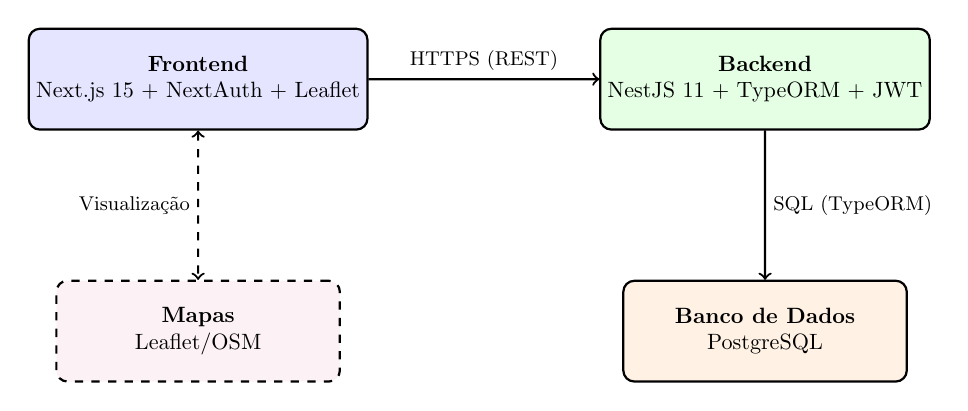
\begin{tikzpicture}[scale=0.8, every node/.style={transform shape}]
  \tikzumlset{font=\footnotesize}
  % Blocos
  \node[draw, rounded corners, thick, fill=blue!10, minimum width=4.5cm, minimum height=1.6cm, align=center] (fe) at (0,2) {\textbf{Frontend}\\Next.js 15 + NextAuth + Leaflet};
  \node[draw, rounded corners, thick, fill=green!10, minimum width=4.5cm, minimum height=1.6cm, align=center] (be) at (9,2) {\textbf{Backend}\\NestJS 11 + TypeORM + JWT};
  \node[draw, rounded corners, thick, fill=orange!10, minimum width=4.5cm, minimum height=1.6cm, align=center] (db) at (9,-2) {\textbf{Banco de Dados}\\PostgreSQL};
  \node[draw, dashed, rounded corners, thick, fill=purple!5, minimum width=4.5cm, minimum height=1.6cm, align=center] (maps) at (0,-2) {\textbf{Mapas}\\Leaflet/OSM};

  % Conexões
  \draw[->, thick] (fe) -- node[above, font=\small]{HTTPS (REST)} (be);
  \draw[->, thick] (be) -- node[right, font=\small]{SQL (TypeORM)} (db);
  \draw[<->, thick, dashed] (fe) -- node[left, font=\small]{Visualização} (maps);
\end{tikzpicture}
\caption{Visão de alto nível da solução.}
\end{figure}

\section{Modelagem do Banco de Dados}
O modelo de dados foi projetado para refletir as agregações de negócio. A Tabela~\ref{tab:principais-entidades} sumariza as principais entidades e seus papéis. De forma geral, todas as entidades operacionais são associadas a uma empresa (\textit{multi-tenancy} por chave estrangeira \texttt{company\_id}). Rotas possuem paradas ordenadas (\texttt{route\_stops}) e agenda de operação (\texttt{route\_schedules}); viagens instanciam rotas em horários específicos e originam bilhetes.

\begin{table}[H]
\centering
\begin{tabular}{ll}
\toprule
\textbf{Entidade} & \textbf{Descrição resumida} \\
\midrule
\texttt{companies} & Empresa (razão social, nome fantasia, CNPJ, slug, contato) \\
\texttt{users} & Usuário (nome, e-mail, senha, papel, status, \texttt{company\_id}) \\
\texttt{drivers} & Motorista (CPF, CNH, categoria, status, \texttt{company\_id}) \\
\texttt{vehicles} & Veículo (placa, capacidade, categoria, status, \texttt{company\_id}) \\
\texttt{addresses} & Endereço (CEP, logradouro, geocoordenadas) \\
\texttt{stops} & Parada (nome, \texttt{address\_id}, acessibilidade, \texttt{company\_id}) \\
\texttt{routes} & Rota (nome, distância, duração estimada, \texttt{company\_id}) \\
\texttt{route\_stops} & Associação rota–parada com ordem e horário opcional \\
\texttt{route\_schedules} & Agenda por dia da semana para a rota \\
\texttt{trips} & Viagem (rota, janelas horárias, status, assentos, \texttt{company\_id}) \\
\texttt{tickets} & Bilhete (passageiro, preço, assento, pontos de embarque) \\
\bottomrule
\end{tabular}
\caption{Principais entidades do domínio.}
\label{tab:principais-entidades}
\end{table}

O diagrama de classes da Figura~\ref{fig:uml-dominio} sintetiza os relacionamentos mais relevantes do domínio.

\begin{figure}[H]
\centering
\begin{tikzpicture}[scale=0.4, every node/.style={transform shape}]
  \tikzumlset{font=\tiny}
  
  % NÍVEL 1: Empresa (topo da hierarquia)
  \umlclass[x=18,y=25]{Company}{
    id: uuid\\
    legalName: string\\
    tradeName: string\\
    slug: string\\
    cnpj: string\\
    email: string\\
    phone: string\\
    logoUrl: string\\
    createdAt: Date\\
    updatedAt: Date
  }{ }
  
  % NÍVEL 2: Gestão de usuários e recursos
  \umlclass[x=3,y=18]{User}{
    id: uuid\\
    name: string\\
    email: string\\
    phone: string\\
    photoUrl: string\\
    password: string\\
    role: UserRole\\
    status: UserStatus\\
    companyId: uuid\\
    createdAt: Date\\
    updatedAt: Date
  }{ }
  
  \umlclass[x=18,y=18]{Vehicle}{
    id: uuid\\
    plate: string\\
    model: string\\
    brand: string\\
    year: number\\
    capacity: number\\
    category: VehicleCategory\\
    comfortConfiguration: ComfortConfiguration\\
    busType: BusType\\
    acquisitionDate: Date\\
    odometer: number\\
    lastMaintenance: Date\\
    nextMaintenance: Date\\
    status: VehicleStatus\\
    notes: string\\
    companyId: uuid
  }{ }
  
  \umlclass[x=33,y=18]{Driver}{
    id: uuid\\
    name: string\\
    cpf: string\\
    licenseNumber: string\\
    licenseCategory: string\\
    licenseExpiry: Date\\
    phone: string\\
    email: string\\
    birthDate: Date\\
    hireDate: Date\\
    status: DriverStatus\\
    emergencyContactName: string\\
    emergencyContactPhone: string\\
    address: string\\
    notes: string\\
    companyId: uuid
  }{ }
  
  % NÍVEL 3: Configuração de rotas
  \umlclass[x=8,y=11]{Route}{
    id: uuid\\
    name: string\\
    description: string\\
    isActive: boolean\\
    estimatedDuration: string\\
    distance: number\\
    companyId: uuid
  }{ }
  
  \umlclass[x=23,y=11]{Stop}{
    id: uuid\\
    name: string\\
    addressId: uuid\\
    isActive: boolean\\
    hasAccessibility: boolean\\
    hasShelter: boolean\\
    companyId: uuid
  }{ }
  
  \umlclass[x=38,y=11]{Address}{
    id: uuid\\
    cep: string\\
    street: string\\
    number: string\\
    complement: string\\
    neighborhood: string\\
    city: string\\
    state: string\\
    longitude: number\\
    latitude: number\\
    createdAt: Date\\
    updatedAt: Date
  }{ }
  
  % NÍVEL 4: Relacionamentos de configuração
  \umlclass[x=8,y=4]{RouteSchedule}{
    id: uuid\\
    routeId: uuid\\
    dayOfWeek: number\\
    isActive: boolean\\
    createdAt: Date\\
    updatedAt: Date
  }{ }
  
  \umlclass[x=23,y=4]{RouteStop}{
    id: uuid\\
    routeId: uuid\\
    stopId: uuid\\
    order: number\\
    departureTime: string
  }{ }
  
  % NÍVEL 5: Operação - Viagens
  \umlclass[x=3,y=-3]{TripVehicle}{
    id: uuid\\
    tripId: uuid\\
    vehicleId: uuid\\
    primaryDriverId: uuid\\
    secondaryDriverId: uuid\\
    isActive: boolean\\
    observations: string\\
    createdAt: Date\\
    updatedAt: Date
  }{ }
  
  \umlclass[x=18,y=-3]{Trip}{
    id: uuid\\
    routeId: uuid\\
    departureTime: Date\\
    estimatedArrivalTime: Date\\
    actualDepartureTime: Date\\
    actualArrivalTime: Date\\
    status: TripStatus\\
    basePrice: number\\
    totalSeats: number\\
    availableSeats: number\\
    isAutoGenerated: boolean\\
    observations: string\\
    companyId: uuid\\
    createdAt: Date\\
    updatedAt: Date
  }{ }
  
  % NÍVEL 6: Vendas - Bilhetes
  \umlclass[x=33,y=-3]{Ticket}{
    id: uuid\\
    tripId: uuid\\
    passengerName: string\\
    passengerDocument: string\\
    passengerPhone: string\\
    passengerEmail: string\\
    seatNumber: string\\
    price: number\\
    status: TicketStatus\\
    boardingPointType: BoardingPointType\\
    boardingStopId: uuid\\
    boardingLocationDescription: string\\
    boardingLatitude: number\\
    boardingLongitude: number\\
    landingPointType: BoardingPointType\\
    landingStopId: uuid\\
    landingLocationDescription: string\\
    landingLatitude: number\\
    landingLongitude: number\\
    observations: string\\
    companyId: uuid
  }{ }

  % RELACIONAMENTOS HIERÁRQUICOS PRINCIPAIS
  % Company -> Recursos
  \umlassoc[mult1=1,mult2=*]{Company}{User}
  \umlassoc[mult1=1,mult2=*]{Company}{Vehicle}
  \umlassoc[mult1=1,mult2=*]{Company}{Driver}
  
  % Company -> Configuração
  \umlassoc[mult1=1,mult2=*,arm1=-135,arm2=90]{Company}{Route}
  \umlassoc[mult1=1,mult2=*,arm1=-45,arm2=90]{Company}{Stop}
  
  % Configuração de endereços
  \umlassoc[mult1=1,mult2=*]{Address}{Stop}
  
  % FLUXO PRINCIPAL: Route -> RouteStop <- Stop
  \umlassoc[mult1=1,mult2=*]{Route}{RouteStop}
  \umlassoc[mult1=1,mult2=*]{Stop}{RouteStop}
  
  % Horários das rotas
  \umlassoc[mult1=1,mult2=*]{Route}{RouteSchedule}
  
  % FLUXO OPERACIONAL: Route -> Trip
  \umlassoc[mult1=1,mult2=*]{Route}{Trip}
  \umlassoc[mult1=1,mult2=*,arm1=-135,arm2=90]{Company}{Trip}
  
  % Trip -> TripVehicle (associação veículo/motorista)
  \umlassoc[mult1=1,mult2=*]{Trip}{TripVehicle}
  \umlassoc[mult1=1,mult2=*,arm1=-90,arm2=90]{Vehicle}{TripVehicle}
  \umlassoc[mult1=1,mult2=*,arm1=-90,arm2=135,stereo=<<primaryDriver>>]{Driver}{TripVehicle}
  
  % FLUXO DE VENDAS: Trip -> Ticket
  \umlassoc[mult1=1,mult2=*]{Trip}{Ticket}
  \umlassoc[mult1=1,mult2=*,arm1=-45,arm2=135]{Company}{Ticket}
  
  % Relacionamento opcional: Stop -> Ticket (embarque/desembarque específico)
  \umldep[stereo=<<boarding/landing>>,mult1=0..1,mult2=*,arm1=-90,arm2=135]{Stop}{Ticket}
  
\end{tikzpicture}
\caption{Diagrama de classes detalhado do domínio BusLy.}
\label{fig:uml-dominio}
\end{figure}

\subsection{Diagramas UML Fracionados por Agregado}
Para facilitar a leitura, os diagramas a seguir detalham os principais agregados do domínio.

\subsubsection*{Agregado Organizacional: Empresas e Usuários}
\begin{figure}[H]
\centering
\begin{tikzpicture}[scale=0.8, every node/.style={transform shape}]
  \tikzumlset{font=\tiny}
  \umlclass[x=0,y=0]{Company}{
    id: uuid\\
    legalName: string\\
    tradeName: string\\
    slug: string\\
    cnpj: string\\
    email: string\\
    phone: string\\
    logoUrl: string\\
    createdAt: Date\\
    updatedAt: Date
  }{ }
  \umlclass[x=8,y=0]{User}{
    id: uuid\\
    name: string\\
    email: string\\
    phone: string\\
    photoUrl: string\\
    password: string\\
    role: UserRole\\
    status: UserStatus\\
    companyId: uuid\\
    createdAt: Date\\
    updatedAt: Date
  }{ }
  \umlassoc[mult1=1,mult2=*]{Company}{User}
  \umlnote[x=0,y=-4, width=12cm]{Company}{Escopo multiempresa: todas as entidades operacionais possuem \texttt{companyId} para isolamento de dados}
\end{tikzpicture}
\caption{Agregado organizacional - estrutura multiempresa.}
\end{figure}

\subsubsection*{Agregado de Rotas e Paradas}
\begin{figure}[H]
\centering
\begin{tikzpicture}[scale=0.7, every node/.style={transform shape}]
  \tikzumlset{font=\tiny}
  \umlclass[x=0,y=2]{Address}{
    id: uuid\\
    cep: string\\
    street: string\\
    number: string\\
    complement: string\\
    neighborhood: string\\
    city: string\\
    state: string\\
    latitude: number\\
    longitude: number\\
    createdAt: Date\\
    updatedAt: Date
  }{ }
  \umlclass[x=8,y=2]{Stop}{
    id: uuid\\
    name: string\\
    addressId: uuid\\
    isActive: boolean\\
    hasAccessibility: boolean\\
    hasShelter: boolean\\
    companyId: uuid
  }{ }
  \umlclass[x=0,y=-3]{RouteSchedule}{
    id: uuid\\
    routeId: uuid\\
    dayOfWeek: number\\
    isActive: boolean\\
    createdAt: Date\\
    updatedAt: Date
  }{ }
  \umlclass[x=6,y=-3]{Route}{
    id: uuid\\
    name: string\\
    description: string\\
    isActive: boolean\\
    estimatedDuration: string\\
    distance: number\\
    companyId: uuid
  }{ }
  \umlclass[x=12,y=-3]{RouteStop}{
    id: uuid\\
    routeId: uuid\\
    stopId: uuid\\
    order: number\\
    departureTime: string
  }{ }
  \umlassoc[mult1=1,mult2=*]{Address}{Stop}
  \umlassoc[mult1=1,mult2=*]{Route}{RouteStop}
  \umlassoc[mult1=1,mult2=*]{Stop}{RouteStop}
  \umlassoc[mult1=1,mult2=*]{Route}{RouteSchedule}
  \umlnote[x=4,y=-6, width=10cm]{Route}{RouteStop implementa relacionamento many-to-many entre Route e Stop com ordem e horários específicos}
\end{tikzpicture}
\caption{Agregado de configuração de rotas, paradas e horários.}
\end{figure}

\subsubsection*{Agregado de Recursos Operacionais}
\begin{figure}[H]
\centering
\begin{tikzpicture}[scale=0.7, every node/.style={transform shape}]
  \tikzumlset{font=\tiny}
  \umlclass[x=0,y=2]{Vehicle}{
    id: uuid\\
    plate: string\\
    model: string\\
    brand: string\\
    year: number\\
    capacity: number\\
    category: VehicleCategory\\
    comfortConfiguration: ComfortConfiguration\\
    busType: BusType\\
    acquisitionDate: Date\\
    odometer: number\\
    lastMaintenance: Date\\
    nextMaintenance: Date\\
    status: VehicleStatus\\
    notes: string\\
    companyId: uuid
  }{ }
  \umlclass[x=15,y=2]{Driver}{
    id: uuid\\
    name: string\\
    cpf: string\\
    licenseNumber: string\\
    licenseCategory: string\\
    licenseExpiry: Date\\
    phone: string\\
    email: string\\
    birthDate: Date\\
    hireDate: Date\\
    status: DriverStatus\\
    emergencyContactName: string\\
    emergencyContactPhone: string\\
    address: string\\
    notes: string\\
    companyId: uuid
  }{ }
  \umlclass[x=7.5,y=-2]{TripVehicle}{
    id: uuid\\
    tripId: uuid\\
    vehicleId: uuid\\
    primaryDriverId: uuid\\
    secondaryDriverId: uuid\\
    isActive: boolean\\
    observations: string\\
    createdAt: Date\\
    updatedAt: Date
  }{ }
  \umlassoc[mult1=1,mult2=*]{Vehicle}{TripVehicle}
  \umlassoc[mult1=1,mult2=*,stereo=<<primaryDriver>>]{Driver}{TripVehicle}
  \umlnote[x=2,y=-6, width=16cm]{TripVehicle}{TripVehicle associa dinamicamente veículos e motoristas às viagens. Um veículo pode ter motorista principal e secundário por viagem}
\end{tikzpicture}
\caption{Agregado de recursos operacionais - frota e motoristas.}
\end{figure}

\subsubsection*{Agregado de Operação e Vendas}
\begin{figure}[H]
\centering
\begin{tikzpicture}[scale=0.6, every node/.style={transform shape}]
  \tikzumlset{font=\tiny}
  \umlclass[x=6,y=3]{Trip}{
    id: uuid\\
    routeId: uuid\\
    departureTime: Date\\
    estimatedArrivalTime: Date\\
    actualDepartureTime: Date\\
    actualArrivalTime: Date\\
    status: TripStatus\\
    basePrice: number\\
    totalSeats: number\\
    availableSeats: number\\
    isAutoGenerated: boolean\\
    observations: string\\
    companyId: uuid\\
    createdAt: Date\\
    updatedAt: Date
  }{ }
  \umlclass[x=0,y=0]{TripVehicle}{
    id: uuid\\
    tripId: uuid\\
    vehicleId: uuid\\
    primaryDriverId: uuid\\
    secondaryDriverId: uuid\\
    isActive: boolean\\
    observations: string\\
    createdAt: Date\\
    updatedAt: Date
  }{ }
  \umlclass[x=12,y=0]{Ticket}{
    id: uuid\\
    tripId: uuid\\
    passengerName: string\\
    passengerDocument: string\\
    passengerPhone: string\\
    passengerEmail: string\\
    seatNumber: string\\
    price: number\\
    status: TicketStatus\\
    boardingPointType: BoardingPointType\\
    boardingStopId: uuid\\
    boardingLocationDescription: string\\
    landingPointType: BoardingPointType\\
    landingStopId: uuid\\
    landingLocationDescription: string\\
    observations: string\\
    companyId: uuid
  }{ }
  \umlclass[x=18,y=3]{Stop}{
    id: uuid\\
    name: string\\
    companyId: uuid
  }{ }
  \umlassoc[mult1=1,mult2=*]{Trip}{TripVehicle}
  \umlassoc[mult1=1,mult2=*]{Trip}{Ticket}
  \umldep[stereo=<<boarding/landing>>,mult1=0..1,mult2=*]{Stop}{Ticket}
  \umlnote[x=1,y=-4, width=14cm]{Trip}{TripVehicle associa veículos e motoristas às viagens. Ticket permite embarque/desembarque em paradas específicas ou localizações customizadas}
\end{tikzpicture}
\caption{Agregado de operação - viagens, recursos e vendas.}
\end{figure}

\section{Arquitetura do Backend}

O backend implementa uma arquitetura modular baseada no framework NestJS 11, seguindo os princípios de \textit{Separation of Concerns} e \textit{Dependency Injection}. A aplicação é estruturada em 10 módulos de domínio, com camadas bem definidas de segurança, validação e persistência.

\subsection{Organização Modular}

O sistema está organizado em três grupos funcionais de módulos, conforme ilustrado na Figura~\ref{fig:backend-modules}.

\begin{figure}[H]
\centering
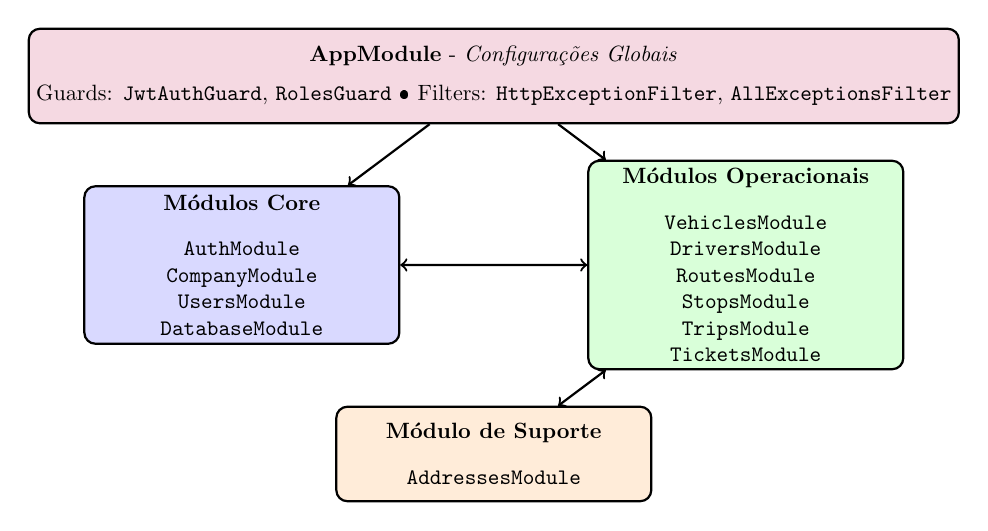
\begin{tikzpicture}[scale=0.8, every node/.style={transform shape}]
  % Módulos Core
  \node[draw, rounded corners, thick, fill=blue!15, minimum width=5cm, minimum height=2.5cm, align=center] (core) at (0,3) {
    \textbf{Módulos Core}\\[0.3cm]
    \texttt{AuthModule}\\
    \texttt{CompanyModule}\\
    \texttt{UsersModule}\\
    \texttt{DatabaseModule}
  };
  
  % Módulos Operacionais
  \node[draw, rounded corners, thick, fill=green!15, minimum width=5cm, minimum height=3cm, align=center] (operational) at (8,3) {
    \textbf{Módulos Operacionais}\\[0.3cm]
    \texttt{VehiclesModule}\\
    \texttt{DriversModule}\\
    \texttt{RoutesModule}\\
    \texttt{StopsModule}\\
    \texttt{TripsModule}\\
    \texttt{TicketsModule}
  };
  
  % Módulos de Suporte
  \node[draw, rounded corners, thick, fill=orange!15, minimum width=5cm, minimum height=1.5cm, align=center] (support) at (4,0) {
    \textbf{Módulo de Suporte}\\[0.3cm]
    \texttt{AddressesModule}
  };
  
  % AppModule
  \node[draw, rounded corners, thick, fill=purple!15, minimum width=10cm, minimum height=1.5cm, align=center] (app) at (4,6) {
    \textbf{AppModule} - \textit{Configurações Globais}\\[0.2cm]
    Guards: \texttt{JwtAuthGuard}, \texttt{RolesGuard} • Filters: \texttt{HttpExceptionFilter}, \texttt{AllExceptionsFilter}
  };
  
  % Setas
  \draw[->, thick] (app) -- (core);
  \draw[->, thick] (app) -- (operational);
  \draw[<->, thick] (core) -- (operational);
  \draw[<->, thick] (support) -- (operational);
\end{tikzpicture}
\caption{Organização modular do backend BusLy.}
\label{fig:backend-modules}
\end{figure}

A organização modular agrupa os componentes por responsabilidade funcional. Os \textbf{Módulos Core} gerenciam autenticação, usuários, empresas e configuração de banco de dados. Os \textbf{Módulos Operacionais} implementam as regras de negócio específicas do domínio de transporte. O \textbf{Módulo de Suporte} fornece funcionalidades auxiliares como geocodificação. O \texttt{AppModule} centraliza as configurações globais de segurança e tratamento de erros, aplicadas a todos os módulos.

\subsection{Pipeline de Processamento}

Cada requisição HTTP passa por um pipeline estruturado de middleware, guards, interceptors e filters, garantindo segurança e consistência.

\begin{figure}[H]
\centering
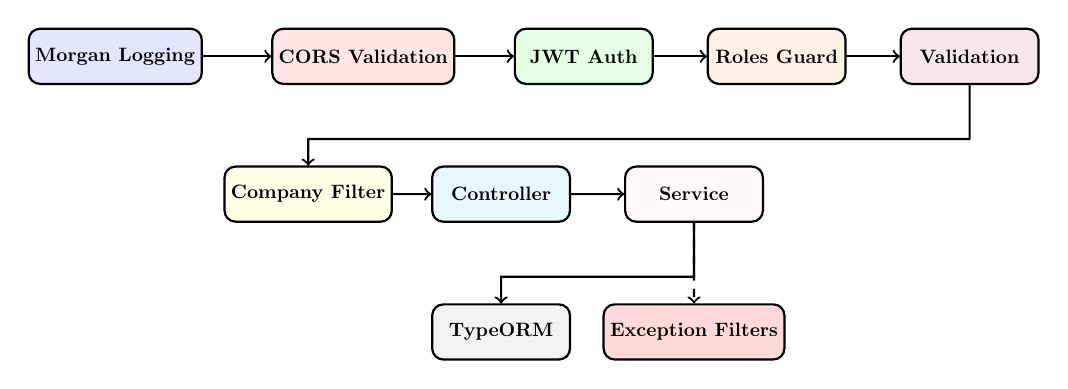
\begin{tikzpicture}[scale=0.7, every node/.style={transform shape}]
  % Pipeline stages
  \node[draw, rounded corners, thick, fill=blue!10, minimum width=2.5cm, minimum height=1cm] (morgan) at (0,0) {\textbf{Morgan Logging}};
  \node[draw, rounded corners, thick, fill=red!10, minimum width=2.5cm, minimum height=1cm] (cors) at (4.5,0) {\textbf{CORS Validation}};
  \node[draw, rounded corners, thick, fill=green!10, minimum width=2.5cm, minimum height=1cm] (jwt) at (8.5,0) {\textbf{JWT Auth}};
  \node[draw, rounded corners, thick, fill=orange!10, minimum width=2.5cm, minimum height=1cm] (roles) at (12,0) {\textbf{Roles Guard}};
  \node[draw, rounded corners, thick, fill=purple!10, minimum width=2.5cm, minimum height=1cm] (validation) at (15.5,0) {\textbf{Validation}};
  
  \node[draw, rounded corners, thick, fill=yellow!10, minimum width=3cm, minimum height=1cm] (interceptor) at (3.5,-2.5) {\textbf{Company Filter}};
  \node[draw, rounded corners, thick, fill=cyan!10, minimum width=2.5cm, minimum height=1cm] (controller) at (7,-2.5) {\textbf{Controller}};
  \node[draw, rounded corners, thick, fill=pink!10, minimum width=2.5cm, minimum height=1cm] (service) at (10.5,-2.5) {\textbf{Service}};
  
  \node[draw, rounded corners, thick, fill=gray!10, minimum width=2.5cm, minimum height=1cm] (typeorm) at (7,-5) {\textbf{TypeORM}};
  \node[draw, rounded corners, thick, fill=red!15, minimum width=3cm, minimum height=1cm] (filters) at (10.5,-5) {\textbf{Exception Filters}};
  
  % Arrows
  \draw[->, thick] (morgan) -- (cors);
  \draw[->, thick] (cors) -- (jwt);
  \draw[->, thick] (jwt) -- (roles);
  \draw[->, thick] (roles) -- (validation);
  \draw[->, thick] (validation) -- ++(0,-1.5) -| (interceptor);
  \draw[->, thick] (interceptor) -- (controller);
  \draw[->, thick] (controller) -- (service);
  \draw[->, thick] (service) -- ++(0,-1.5) -| (typeorm);
  \draw[->, thick, dashed] (service) -- (filters);
\end{tikzpicture}
\caption{Pipeline de processamento de requisições.}
\label{fig:request-pipeline}
\end{figure}

O pipeline garante que cada requisição passe por validações sequenciais obrigatórias. Inicialmente, o \textbf{Morgan} registra logs e o \textbf{CORS} valida origens permitidas. A autenticação via \textbf{JwtAuthGuard} verifica tokens válidos, seguida da autorização por \textbf{RolesGuard} que confirma permissões do usuário. O \textbf{ValidationPipe} valida DTOs de entrada. O \textbf{CompanyFilterInterceptor} injeta o contexto multiempresa antes do processamento pelo \textbf{Controller} e \textbf{Service}. Finalmente, o \textbf{TypeORM} persiste dados e os \textbf{Exception Filters} tratam erros de forma padronizada.

\subsection{Fluxo de Autenticação}

O sistema utiliza autenticação baseada em JWT com suporte a multi-tenancy. A Figura~\ref{fig:auth-sequence} detalha o processo completo.

\begin{figure}[H]
\centering
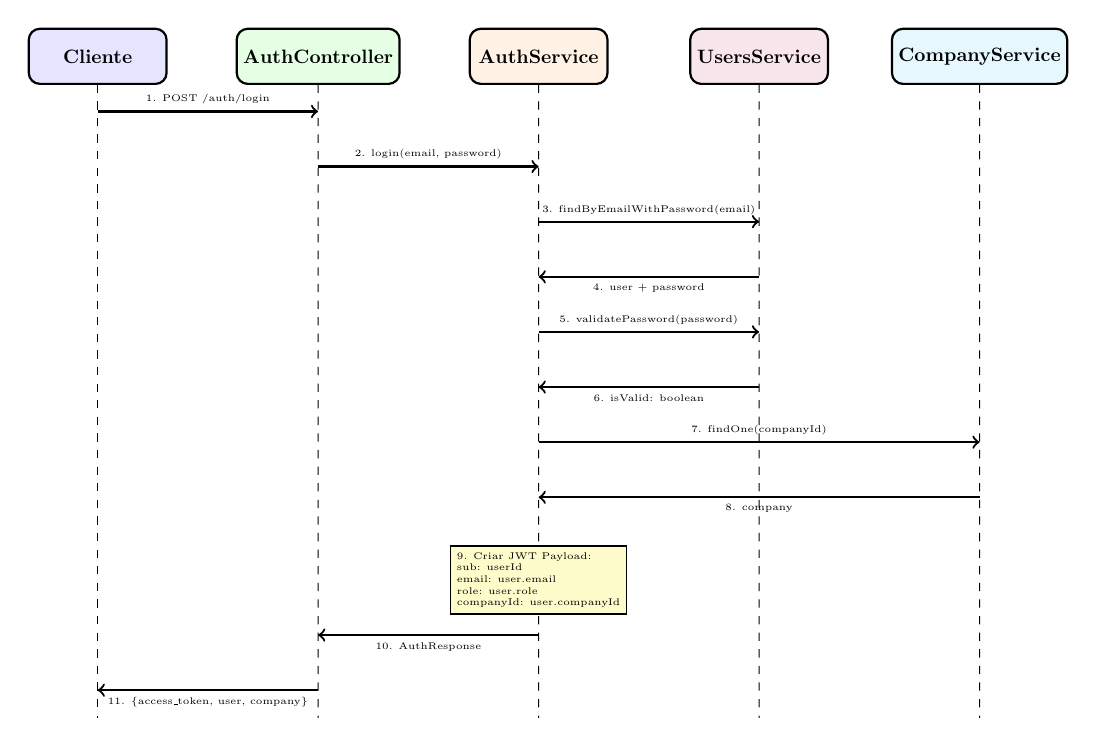
\begin{tikzpicture}[scale=0.7, every node/.style={transform shape}]
  % Participantes
  \node[draw, rounded corners, thick, fill=blue!10, minimum width=2.5cm, minimum height=1cm] (client) at (0,11) {\textbf{Cliente}};
  \node[draw, rounded corners, thick, fill=green!10, minimum width=2.5cm, minimum height=1cm] (auth) at (4,11) {\textbf{AuthController}};
  \node[draw, rounded corners, thick, fill=orange!10, minimum width=2.5cm, minimum height=1cm] (service) at (8,11) {\textbf{AuthService}};
  \node[draw, rounded corners, thick, fill=purple!10, minimum width=2.5cm, minimum height=1cm] (users) at (12,11) {\textbf{UsersService}};
  \node[draw, rounded corners, thick, fill=cyan!10, minimum width=2.5cm, minimum height=1cm] (company) at (16,11) {\textbf{CompanyService}};
  
  % Linhas de vida
  \draw[dashed] (client) -- (0,-1);
  \draw[dashed] (auth) -- (4,-1);
  \draw[dashed] (service) -- (8,-1);
  \draw[dashed] (users) -- (12,-1);
  \draw[dashed] (company) -- (16,-1);
  
  % Mensagens
  \draw[->, thick] (0,10) -- node[above, font=\tiny]{1. POST /auth/login} (4,10);
  \draw[->, thick] (4,9) -- node[above, font=\tiny]{2. login(email, password)} (8,9);
  \draw[->, thick] (8,8) -- node[above, font=\tiny]{3. findByEmailWithPassword(email)} (12,8);
  \draw[<-, thick] (8,7) -- node[below, font=\tiny]{4. user + password} (12,7);
  \draw[->, thick] (8,6) -- node[above, font=\tiny]{5. validatePassword(password)} (12,6);
  \draw[<-, thick] (8,5) -- node[below, font=\tiny]{6. isValid: boolean} (12,5);
  \draw[->, thick] (8,4) -- node[above, font=\tiny]{7. findOne(companyId)} (16,4);
  \draw[<-, thick] (8,3) -- node[below, font=\tiny]{8. company} (16,3);
  
  % Processamento interno
  \node[draw, fill=yellow!20, align=left, font=\tiny] at (8,1.5) {9. Criar JWT Payload:\\sub: userId\\email: user.email\\role: user.role\\companyId: user.companyId};
  
  \draw[<-, thick] (4,0.5) -- node[below, font=\tiny]{10. AuthResponse} (8,0.5);
  \draw[<-, thick] (0,-0.5) -- node[below, font=\tiny]{11. \{access\_token, user, company\}} (4,-0.5);
\end{tikzpicture}
\caption{Diagrama de sequência - fluxo de autenticação.}
\label{fig:auth-sequence}
\end{figure}

O fluxo de autenticação implementa um processo seguro e eficiente em 11 etapas. O cliente envia credenciais via POST para o \texttt{AuthController}, que delega ao \texttt{AuthService} a validação. O \texttt{UsersService} busca o usuário por email (incluindo senha hash), valida a senha fornecida e retorna o resultado. Confirmada a autenticação, o \texttt{AuthService} consulta os dados da empresa via \texttt{CompanyService} e cria o payload JWT contendo informações do usuário e contexto empresarial. A resposta final inclui o token de acesso, dados do usuário e informações da empresa, permitindo que o frontend mantenha o contexto de sessão multiempresa.

\subsection{Arquitetura Multi-tenant}

O sistema implementa isolamento de dados por empresa através do padrão \texttt{BaseCompanyService}, que injeta automaticamente o \texttt{companyId} em todas as operações de banco de dados. O \texttt{CompanyFilterInterceptor} extrai o contexto da empresa do token JWT e disponibiliza para os serviços.

\begin{itemize}
  \item \textbf{Isolamento Automático}: Todas as entidades operacionais possuem \texttt{companyId}
  \item \textbf{Herança de Comportamento}: Services estendem \texttt{BaseCompanyService<T>}
  \item \textbf{Contexto de Requisição}: Interceptor injeta \texttt{companyId} baseado no token JWT
  \item \textbf{Validação de Acesso}: Queries automáticas com filtro por empresa
\end{itemize}

\section{Arquitetura do Frontend}

O frontend implementa uma arquitetura moderna baseada em Next.js~15 (React~19) com App Router, utilizando TypeScript para tipagem estática completa. A aplicação segue padrões de arquitetura limpa e organização por domínio.

\subsection{Stack Tecnológico e Organização}

O frontend utiliza um conjunto integrado de tecnologias modernas para garantir performance, experiência do usuário e manutenibilidade:

\begin{itemize}
  \item \textbf{Framework}: Next.js~15 com App Router para roteamento baseado em arquivo
  \item \textbf{UI}: React~19 com componentes Radix UI e estilização Tailwind CSS
  \item \textbf{Formulários}: React Hook Form + Zod para validação tipada
  \item \textbf{Autenticação}: NextAuth v4 com JWT e provedores customizados
  \item \textbf{Mapas}: Leaflet + React-Leaflet para funcionalidades geográficas
  \item \textbf{Estado}: Context API do React para gerenciamento de estado global
  \item \textbf{Tipagem}: TypeScript com definições específicas por domínio
\end{itemize}

\subsection{Arquitetura de Roteamento}

A aplicação utiliza o App Router do Next.js~15 com roteamento dinâmico baseado em empresa. A estrutura principal segue o padrão \texttt{/dashboard/[company]/recurso}, permitindo isolamento completo por empresa:

\begin{itemize}
  \item \textbf{Páginas Públicas}: \texttt{/login}, \texttt{/criar-empresa}
  \item \textbf{Dashboard Multiempresa}: \texttt{/dashboard/[company]/\{motoristas, veiculos, rotas, paradas, viagens, passagens\}}
  \item \textbf{Layouts Aninhados}: Cada nível possui layout específico com providers e componentes apropriados
  \item \textbf{Proteção de Rotas}: Wrapper \texttt{ProtectedPage} valida autenticação e autorização
\end{itemize}

\subsection{Gerenciamento de Estado e Contextos}

O sistema implementa uma hierarquia de contextos React para gerenciar estado global de forma eficiente:

\begin{figure}[H]
\centering
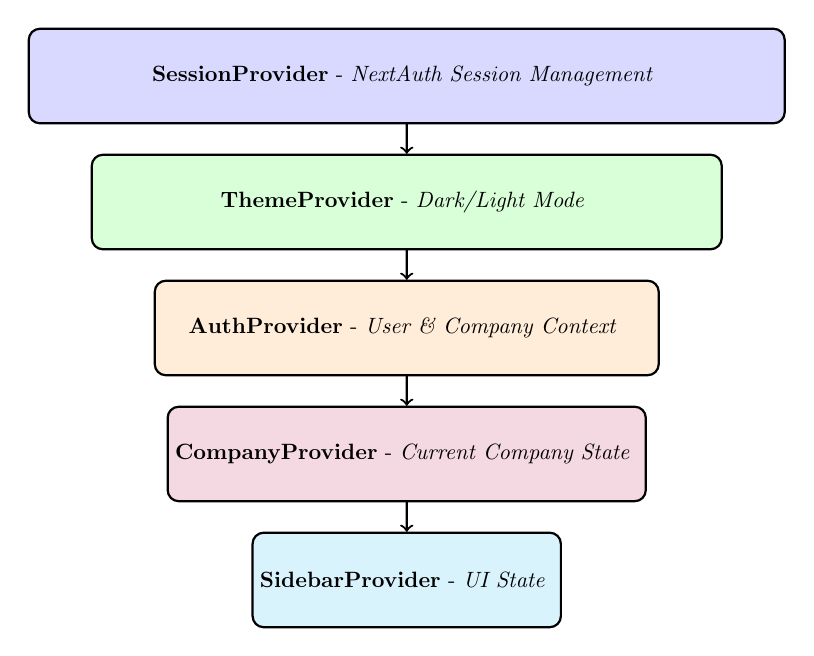
\begin{tikzpicture}[scale=0.8, every node/.style={transform shape}]
  % Providers hierarchy
  \node[draw, rounded corners, thick, fill=blue!15, minimum width=12cm, minimum height=1.5cm, align=center] (session) at (6,6) {
    \textbf{SessionProvider} - \textit{NextAuth Session Management}
  };
  
  \node[draw, rounded corners, thick, fill=green!15, minimum width=10cm, minimum height=1.5cm, align=center] (theme) at (6,4) {
    \textbf{ThemeProvider} - \textit{Dark/Light Mode}
  };
  
  \node[draw, rounded corners, thick, fill=orange!15, minimum width=8cm, minimum height=1.5cm, align=center] (auth) at (6,2) {
    \textbf{AuthProvider} - \textit{User \& Company Context}
  };
  
  \node[draw, rounded corners, thick, fill=purple!15, minimum width=6cm, minimum height=1.5cm, align=center] (company) at (6,0) {
    \textbf{CompanyProvider} - \textit{Current Company State}
  };
  
  \node[draw, rounded corners, thick, fill=cyan!15, minimum width=4cm, minimum height=1.5cm, align=center] (sidebar) at (6,-2) {
    \textbf{SidebarProvider} - \textit{UI State}
  };
  
  % Arrows showing hierarchy
  \draw[->, thick] (session) -- (theme);
  \draw[->, thick] (theme) -- (auth);
  \draw[->, thick] (auth) -- (company);
  \draw[->, thick] (company) -- (sidebar);
\end{tikzpicture}
\caption{Hierarquia de providers e contextos do frontend.}
\label{fig:frontend-providers}
\end{figure}

Cada contexto tem responsabilidades específicas:

\begin{itemize}
  \item \textbf{SessionProvider}: Gerencia sessão NextAuth e tokens JWT
  \item \textbf{AuthProvider}: Expõe dados do usuário autenticado e empresa
  \item \textbf{CompanyProvider}: Mantém contexto da empresa atual no dashboard
  \item \textbf{ThemeProvider}: Controla tema dark/light com persistência
  \item \textbf{SidebarProvider}: Gerencia estado da interface (sidebar, mobile)
\end{itemize}

\subsection{Sistema de Autenticação e Comunicação}

A autenticação integra NextAuth com o backend NestJS através de JWT. O serviço \texttt{api.service.ts} centraliza toda comunicação HTTP:

\begin{itemize}
  \item \textbf{Token Management}: Anexa automaticamente \texttt{Bearer} tokens
  \item \textbf{Error Handling}: Trata respostas de erro padronizadas e redireciona em 401
  \item \textbf{Response Processing}: Extrai dados da estrutura padrão da API
  \item \textbf{Public Endpoints}: Diferencia rotas que não requerem autenticação
  \item \textbf{Session Validation}: Verifica validade da sessão antes de cada requisição
\end{itemize}

\subsection{Arquitetura de Componentes}

O sistema de componentes segue uma arquitetura em camadas baseada em responsabilidades:

\begin{itemize}
  \item \textbf{Primitivos UI}: Radix UI como base para acessibilidade e comportamento
  \item \textbf{Design System}: Componentes tipados (\texttt{components/ui/}) com variantes via CVA
  \item \textbf{Componentes de Domínio}: Específicos por funcionalidade (forms, tables, dialogs)
  \item \textbf{Páginas}: Composição de componentes com lógica de negócio específica
  \item \textbf{Layouts}: Estruturas reutilizáveis com providers e navegação
\end{itemize}

\subsection{Tipagem e Validação}

O TypeScript é utilizado extensivamente com tipagem específica por domínio:

\begin{itemize}
  \item \textbf{Types Directory}: Definições tipadas por entidade (\texttt{User}, \texttt{Company}, \texttt{Vehicle}, etc.)
  \item \textbf{API Responses}: Tipos padronizados para respostas da API
  \item \textbf{Form Validation}: Schemas Zod para validação client-side
  \item \textbf{Service Layer}: Métodos tipados para cada endpoint da API
  \item \textbf{NextAuth Extension}: Tipos customizados para sessão e JWT payload
\end{itemize}

Esta arquitetura garante: (i) separação clara de responsabilidades, (ii) tipagem estática end-to-end, (iii) reutilização de componentes, (iv) experiência consistente multiempresa e (v) escalabilidade via modularização por domínio.

\chapter{Módulos e Funcionalidades do Frontend}

O frontend do sistema BusLy oferece uma interface moderna e intuitiva para gestão completa de operações de transporte rodoviário. A aplicação é desenvolvida em Next.js~15 com React~19, proporcionando uma experiência de usuário fluida e responsiva.

\section{Autenticação e Gestão de Empresa}

\subsection{Tela de Login e Registro}

A autenticação do sistema é realizada através de uma interface limpa e moderna. A tela de login apresenta campos para email e senha, com validação em tempo real e feedback visual para o usuário. O sistema utiliza NextAuth v4 para gerenciamento de sessão, garantindo segurança e persistência do estado de autenticação.

\begin{figure}[H]
  \centering
  \includegraphics[width=0.8\textwidth]{imagens/tela-login.png}
  \caption{Tela de login do sistema BusLy.}
  \label{fig:tela-login}
\end{figure}

\subsection{Fluxo de Criação da Empresa}

Após o primeiro acesso, usuários sem empresa associada são direcionados para o fluxo de criação de empresa. Este processo inclui cadastro da empresa com informações básicas (nome, CNPJ, endereço), configuração inicial de parâmetros operacionais e validação automática de dados.

\begin{figure}[H]
  \centering
  \includegraphics[width=0.8\textwidth]{imagens/criacao-empresa.png}
  \caption{Formulário de criação de empresa.}
  \label{fig:criacao-empresa}
\end{figure}

\section{Painel de Controle (Dashboard)}

O dashboard principal oferece uma visão consolidada das operações da empresa, apresentando métricas importantes e acesso rápido aos módulos principais.

\subsection{Visão Geral}

O painel de controle exibe cards informativos com estatísticas em tempo real: total de viagens, passagens vendidas, veículos ativos, motoristas disponíveis, rotas ativas e paradas cadastradas.

\begin{figure}[H]
  \centering
  \includegraphics[width=0.9\textwidth]{imagens/dashboard.png}
  \caption{Painel de controle principal com métricas e navegação.}
  \label{fig:dashboard}
\end{figure}

\section{Módulo de Paradas}

O módulo de paradas permite o cadastro e gerenciamento de pontos de embarque e desembarque, com integração a mapas interativos.

\subsection{Listagem de Paradas}

A tela de listagem apresenta todas as paradas cadastradas em formato de tabela, com funcionalidades de busca, filtros e ações rápidas (editar, visualizar, excluir).

\begin{figure}[H]
  \centering
  \includegraphics[width=0.9\textwidth]{imagens/listagem-paradas.png}
  \caption{Listagem de paradas com funcionalidades de busca e filtros.}
  \label{fig:listagem-paradas}
\end{figure}

\subsection{Criação e Edição de Paradas}

O formulário de cadastro de paradas integra um mapa interativo baseado em Leaflet, permitindo seleção geográfica por clique, arrastar marcador para ajuste fino, validação de endereço e informações detalhadas como nome, descrição e horários de funcionamento.

\begin{figure}[H]
  \centering
  \includegraphics[width=0.9\textwidth]{imagens/formulario-parada.png}
  \caption{Formulário de cadastro de parada com mapa interativo.}
  \label{fig:formulario-parada}
\end{figure}

\section{Módulo de Rotas}

O módulo de rotas permite a criação de itinerários conectando paradas em sequência lógica, incluindo definição de paradas em ordem de visitação, cálculo automático de distâncias e configuração de preços por trecho.

\begin{figure}[H]
  \centering
  \includegraphics[width=0.9\textwidth]{imagens/criacao-rota.png}
  \caption{Interface de criação de rota com seleção de paradas.}
  \label{fig:criacao-rota}
\end{figure}

\section{Módulo de Veículos}

O módulo de veículos gerencia a frota da empresa, permitindo cadastro completo (placa, modelo, capacidade, ano), controle de status operacional (ativo, em manutenção, inativo), histórico de viagens e filtros avançados.

\begin{figure}[H]
  \centering
  \includegraphics[width=0.9\textwidth]{imagens/veiculos.png}
  \caption{Listagem de veículos com status operacional.}
  \label{fig:veiculos}
\end{figure}

\section{Módulo de Motoristas}

O módulo de motoristas gerencia a equipe de condutores, incluindo dados pessoais (nome, CPF, CNH, contatos), informações profissionais (categoria da CNH, experiência), status de disponibilidade e histórico de viagens.

\begin{figure}[H]
  \centering
  \includegraphics[width=0.9\textwidth]{imagens/motoristas.png}
  \caption{Interface de gerenciamento de motoristas.}
  \label{fig:motoristas}
\end{figure}

\section{Módulo de Viagens}

O módulo de viagens permite o agendamento e gerenciamento de viagens através de um fluxo estruturado: seleção da rota, definição de data e horário, associação de veículo, designação de motorista, configuração de preços e confirmação final.

\begin{figure}[H]
  \centering
  \includegraphics[width=0.9\textwidth]{imagens/agendamento-viagem.png}
  \caption{Processo de agendamento de viagem.}
  \label{fig:agendamento-viagem}
\end{figure}

\section{Módulo de Venda de Passagens}

O módulo de passagens implementa um assistente (wizard) intuitivo para venda de passagens, guiando o usuário através de cinco etapas sequenciais.

\subsection{Assistente de Venda de Passagens}

\subsubsection{1. Seleção de Rota}

Primeira etapa com listagem de rotas disponíveis, filtros por data, informações da rota (paradas, horários, preços) e verificação de disponibilidade de assentos.

\begin{figure}[H]
  \centering
  \includegraphics[width=0.9\textwidth]{imagens/wizard-rota.png}
  \caption{Seleção de rota no wizard de passagens.}
  \label{fig:wizard-rota}
\end{figure}

\subsubsection{2. Seleção de Data e Horário}

Segunda etapa com calendário interativo, horários disponíveis e informação de capacidade restante.

\begin{figure}[H]
  \centering
  \includegraphics[width=0.9\textwidth]{imagens/wizard-data.png}
  \caption{Seleção de data e horário.}
  \label{fig:wizard-data}
\end{figure}

\subsubsection{3. Informações do Passageiro}

Terceira etapa para coleta de dados pessoais (nome completo, CPF), contatos (telefone, email) e validação automática de CPF.

\begin{figure}[H]
  \centering
  \includegraphics[width=0.9\textwidth]{imagens/wizard-passageiro.png}
  \caption{Cadastro de informações do passageiro.}
  \label{fig:wizard-passageiro}
\end{figure}

\subsubsection{4. Seleção de Locais de Embarque e Desembarque}

Quarta etapa com seleção de paradas oficiais ou definição de locais personalizados, cálculo de preço baseado na distância e observações para o motorista.

\begin{figure}[H]
  \centering
  \includegraphics[width=0.9\textwidth]{imagens/wizard-locais.png}
  \caption{Seleção de locais de embarque e desembarque.}
  \label{fig:wizard-locais}
\end{figure}

\subsubsection{5. Confirmação e Pagamento}

Etapa final com resumo da viagem, detalhes da passagem, preço final e geração automática do bilhete.

\begin{figure}[H]
  \centering
  \includegraphics[width=0.9\textwidth]{imagens/wizard-confirmacao.png}
  \caption{Confirmação final e geração da passagem.}
  \label{fig:wizard-confirmacao}
\end{figure}

\section{Características da Interface}

\subsection{Design Responsivo}

A interface é totalmente responsiva, adaptando-se a diferentes tamanhos de tela: desktop com layout completo, tablet com adaptação automática e mobile com interface otimizada.

\subsection{Experiência do Usuário}

O sistema prioriza a usabilidade através de navegação intuitiva, feedback visual com notificações e estados de carregamento, validação em tempo real e suporte à acessibilidade.

\subsection{Integração com Mapas}

A integração com mapas interativos (Leaflet) oferece visualização geográfica precisa, seleção por clique, funcionalidade de arrastar e soltar para ajuste fino e controles intuitivos de zoom e navegação.

O frontend do BusLy proporciona uma experiência completa e profissional para gestão de operações de transporte, combinando funcionalidade avançada com interface intuitiva e moderna.




\chapter{Resultados e Discussão}\label{cha:resultados}

\section{Verificação de Requisitos}

A primeira etapa da avaliação consistiu na verificação sistemática do grau de implementação dos Requisitos Funcionais (RF) e Não Funcionais (RNF) definidos no Capítulo 3. A análise buscou constatar se as funcionalidades e características planejadas foram efetivamente traduzidas em software. As Tabelas \ref{tab:verificacao-rf} e \ref{tab:verificacao-rnf} apresentam o resultado consolidado desta verificação.

\begin{table}[htbp]
  \centering
  \caption{Verificação dos Requisitos Funcionais (RF)}
  \label{tab:verificacao-rf}
  \resizebox{\textwidth}{!}{%
    \begin{tabular}{|l|c|p{9.5cm}|}
      \hline
      \textbf{Requisito}             & \textbf{Status}           & \textbf{Observações e Evidências}                                                                        \\
      \hline
      RF01 -- Registro               & Implementado              & Fluxo de cadastro de usuários disponível na API de autenticação, com validação de dados.                 \\
      RF02 -- Login                  & Implementado              & Autenticação via e-mail e senha com emissão de JWT e proteção de rotas.                                  \\
      RF03 -- Permissões             & Implementado              & Controle de acesso por perfis/roles com guards no backend e proteção de rotas no frontend.               \\
      RF04 -- Empresas               & Implementado              & Criação e gestão de perfis de empresa disponíveis; página de criação de empresa no frontend.             \\
      RF05 -- Isolamento             & Implementado              & Interceptor/serviço central aplica filtro por \textit{companyId} do usuário em todas as requisições.     \\
      RF06 -- Motoristas             & Implementado              & CRUD completo de motoristas no módulo dedicado.                                                          \\
      RF07 -- Veículos               & Implementado              & CRUD completo de veículos no módulo dedicado.                                                            \\
      RF08 -- Paradas                & Implementado              & CRUD de pontos de parada com armazenamento de geolocalização.                                            \\
      RF09 -- Rotas                  & Implementado              & Criação e manutenção de rotas com sequência de paradas.                                                  \\
      RF10 -- Horários               & Parcialmente Implementado & Associação de horários e preços às rotas; serviços de \textit{schedules} no frontend.                    \\
      RF11 -- Mapas                  & Parcialmente Implementado & Visualização de rotas e paradas disponível; ausência de mapa interativo avançado em algumas telas.       \\
      RF12 -- Agendamento de Viagens & Implementado              & Criação de viagens baseada em rotas e horários no módulo de viagens.                                     \\
      RF13 -- Atribuição             & Implementado              & Associação de veículos e motoristas às viagens.                                                          \\
      RF14 -- Status de Viagens      & Parcialmente Implementado & Atualização de status disponível; sem comunicação em tempo real por WebSocket.                           \\
      RF15 -- Wizard de Venda        & Implementado              & Fluxo guiado de venda com \textit{wizard} no frontend.                                                   \\
      RF16 -- Embarque/Desembarque   & Implementado              & Seleção flexível de pontos ao longo da rota no ato da venda.                                             \\
      RF17 -- Passageiros            & Implementado              & Coleta e armazenamento dos dados completos dos passageiros.                                              \\
      RF18 -- Anti-Overbooking       & Implementado              & Verificação de disponibilidade antes da emissão; criação de ticket bloqueada com erro 409 quando lotado. \\
      RF19 -- Listas                 & Implementado              & Geração/visualização de listas de passageiros por viagem nas telas operacionais.                         \\
      RF20 -- Busca                  & Parcialmente Implementado & Filtros múltiplos disponíveis nas listagens; oportunidades de ampliar critérios e combinações.           \\
      RF21 -- Ocupação em Tempo Real & Parcialmente Implementado & Visualização de ocupação por viagem; ausência de atualização \textit{push} em tempo real.                \\
      \hline
    \end{tabular}%
  }
\end{table}

\begin{table}[htbp]
  \centering
  \caption{Verificação dos Requisitos Não Funcionais (RNF)}
  \label{tab:verificacao-rnf}
  \resizebox{\textwidth}{!}{%
    \begin{tabular}{|l|c|p{9.5cm}|}
      \hline
      \textbf{Requisito}                  & \textbf{Status}           & \textbf{Observações e Evidências}                                                         \\
      \hline
      RNF01 -- Responsividade             & Implementado              & Interface responsiva, componentes padronizados e adaptação a diferentes tamanhos de tela. \\
      RNF02 -- Navegação                  & Parcialmente Implementado & Fluxos principais claros; avaliação heurística indica melhorias na prevenção de erros.    \\
      RNF03 -- Acessibilidade             & Parcialmente Implementado & Formulários com indicadores de progresso; faltam recursos avançados de acessibilidade.    \\
      RNF04 -- Autenticação               & Implementado              & Login seguro com JWT e controle de sessão.                                                \\
      RNF05 -- Autorização                & Implementado              & Acesso baseado em perfis com guards e verificação centralizada.                           \\
      RNF06 -- Isolamento                 & Implementado              & Separação de dados por empresa garantida via filtro automático por \textit{companyId}.    \\
      RNF07 -- Validação                  & Implementado              & Validação de entrada no backend (DTOs/validators) e no frontend.                          \\
      RNF08 -- Desempenho de Carregamento & Implementado              & Páginas com tempos de resposta adequados nos fluxos críticos.                             \\
      RNF09 -- Otimização de Consultas    & Parcialmente Implementado & Consultas indexadas nos módulos principais; há espaço para otimizações adicionais.        \\
      RNF10 -- Escalabilidade             & Parcialmente Implementado & Arquitetura modular; ausência de escalonamento horizontal automático e fila de mensagens. \\
      RNF11 -- Arquitetura                & Implementado              & Código organizado por módulos com camadas bem definidas.                                  \\
      RNF12 -- Padrões                    & Implementado              & Padrões de codificação consistentes e lint configurado.                                   \\
      RNF13 -- Documentação               & Parcialmente Implementado & Documentação básica presente; falta detalhamento abrangente de API e decisões de projeto. \\
      RNF14 -- Containerização            & Implementado              & Dockerfile no frontend e backend; orquestração via \texttt{docker-compose}.               \\
      RNF15 -- Configuração de Ambientes  & Implementado              & Suporte a múltiplos ambientes com variáveis de ambiente.                                  \\
      \hline
    \end{tabular}%
  }
\end{table}

\section{Avaliação Heurística}
A segunda etapa da avaliação do protótipo consistiu em uma Avaliação Heurística, método de inspeção de usabilidade consolidado por Nielsen (1994). Atuando como avaliador especialista, foram analisados os principais fluxos de interação do sistema, como o cadastro de rotas e a venda de passagens, com o objetivo de identificar potenciais problemas e pontos de aderência a boas práticas de design de interface. A seguir, são discutidos os achados mais relevantes, agrupados pelas heurísticas correspondentes.

Visibilidade do status do sistema (Heurística 1)
O sistema se destaca na aplicação desta heurística. Em operações que demandam tempo, como o carregamento de tabelas de dados, a interface exibe componentes de skeleton loading (Figura X, a ser inserida por você, mostrando a tabela "carregando"), comunicando claramente ao usuário que uma ação está em progresso. Adicionalmente, ações de sucesso ou falha, como salvar um novo veículo, disparam notificações do tipo toast no canto da tela, como ilustrado na Figura \ref{fig:toast-success}, fornecendo feedback imediato e não intrusivo.

Correspondência entre o sistema e o mundo real (Heurística 2)
A plataforma utiliza uma linguagem e iconografia familiar ao usuário-alvo. Termos como "Frota", "Motoristas", "Paradas" e "Rotas" são diretos e correspondem à terminologia do setor. A utilização de mapas interativos para a gestão de paradas e visualização de rotas, como visto na Figura \ref{fig:mapa-paradas}, cria uma representação visual que espelha diretamente a operação logística do mundo real, facilitando o entendimento e a manipulação dos dados.

Consistência e padronização (Heurística 4)
Este é um dos pontos mais fortes do protótipo. A utilização sistemática da biblioteca de componentes shadcn/ui garante uma alta consistência visual e de interação. Elementos como botões, formulários, tabelas e modais, como o de cadastro de nova parada (Figura \ref{fig:modal-parada}), mantêm uma identidade e um comportamento padronizados em todos os módulos. Essa consistência reduz a carga cognitiva do usuário e acelera a curva de aprendizado da ferramenta.

Prevenção de erros (Heurística 5)
Neste ponto, foram identificadas oportunidades de melhoria. No formulário de criação de rotas (Figura \ref{fig:form-rotas}), o sistema atualmente permite que o usuário avance e tente salvar uma rota sem ter selecionado nenhuma parada. Isso representa um erro potencial, pois uma rota sem paradas é funcionalmente inútil e pode gerar dados inconsistentes. Uma melhoria recomendada seria a implementação de uma validação no frontend que desabilite o botão "Salvar" ou exiba uma mensagem de alerta enquanto a lista de paradas da rota estiver vazia.

Reconhecimento em vez de memorização (Heurística 6)
A interface faz um bom trabalho ao manter as opções e informações visíveis. O menu lateral persistente (Figura \ref{fig:sidebar}) permite que o usuário navegue entre os módulos sem precisar memorizar o caminho. No entanto, no fluxo de venda de passagens, o sistema poderia melhorar ao exibir um resumo da seleção (ex: "Rota: Picos x Teresina, Data: 29/08/2025") em todos os passos do assistente, para que o usuário não precise memorizar as informações inseridas nos passos anteriores.

Estética e design minimalista (Heurística 8)
A interface do ViaBus é limpa e funcional. Não há excesso de informações ou elementos visuais que possam distrair o usuário de suas tarefas. O uso de espaços em branco e a hierarquia visual clara, como visto no Dashboard (Figura \ref{fig:dashboard}), contribuem para um design minimalista que prioriza o conteúdo e a funcionalidade.

\section{Discussão dos Resultados}

Lorem ipsum dolor sit amet, consectetur adipiscing elit. Sed do eiusmod tempor incididunt ut labore et dolore magna aliqua. Ut enim ad minim veniam, quis nostrud exercitation ullamco laboris nisi ut aliquip ex ea commodo consequat. Duis aute irure dolor in reprehenderit in voluptate velit esse cillum dolore eu fugiat nulla pariatur. Excepteur sint occaecat cupidatat non proident, sunt in culpa qui officia deserunt mollit anim id est laborum.
\chapter{Considerações Finais}
\label{cha:consideracoes_finais}

Este trabalho de conclusão de curso abordou o desafio da gestão operacional no setor de transporte rodoviário alternativo de passageiros, um segmento caracterizado pela carência de soluções tecnológicas acessíveis. O problema central identificado foi a dependência de métodos manuais e fragmentados, que resultam em ineficiências e risco de erros. Diante deste cenário, o objetivo geral do projeto foi desenvolver um protótipo funcional de uma plataforma web, no modelo \textit{Software as a Service} (SaaS), denominada ViaBus, para centralizar e digitalizar essa gestão.

\section{Conclusão}

Conclui-se que o objetivo geral do trabalho foi atingido, uma vez que o protótipo funcional foi desenvolvido e sua arquitetura, detalhada. A implementação materializou os requisitos essenciais levantados na pesquisa de mercado — como o gerenciamento de recursos e a execução de operações de venda —, demonstrando que a abordagem técnica proposta é uma solução plausível para o problema. As contribuições deste projeto são, portanto, de ordem prática e documental: o próprio protótipo funcional, que serve como prova de conceito, e a documentação de uma proposta de arquitetura para a construção de um sistema SaaS multi-tenant focado neste nicho de mercado.

\section{Limitações do Trabalho}

É fundamental reconhecer as limitações inerentes a este trabalho para contextualizar o alcance de suas conclusões. A principal limitação metodológica reside na pesquisa de mercado, conduzida com uma amostra de apenas dois gestores, o que não permite a generalização estatística dos achados. No que tange à validação, a utilização de uma Avaliação Heurística em vez de testes com usuários finais oferece conclusões de usabilidade de caráter preliminar. Por fim, o escopo do protótipo funcional foi deliberadamente focado na perspectiva do gestor, não incluindo o desenvolvimento de uma aplicação para o passageiro, funcionalidade apontada como relevante na pesquisa.

\section{Trabalhos Futuros}

Com base nas limitações apontadas, delineia-se um caminho claro para a evolução do projeto. Recomenda-se, primeiramente, a validação da solução em maior escala, através de uma pesquisa de mercado quantitativa e da condução de testes de usabilidade com usuários reais. Em paralelo, o desenvolvimento do protótipo pode avançar com a implementação de funcionalidades de relatório (RF11) e do manifesto de viagem para o motorista (RF09). A criação de um aplicativo móvel complementar para o passageiro, permitindo a compra de bilhetes e o rastreamento de viagens, e a integração com sistemas de pagamento online representam os passos subsequentes para transformar o protótipo em um produto de mercado.